
\clearpage
\section{Le classement des documents}
\label{bkm:Ref434830029}\label{bkm:Ref434828324}

\begin{wrapfigure}[14]{l}{6.5cm}   % [x] Wie manche Zeile soll sich um die Grafik "brechen"
  \vspace{-35pt}      % Grundwert war 20; mit 30 schön oben beim Text ausgerichtet
  \begin{center}
    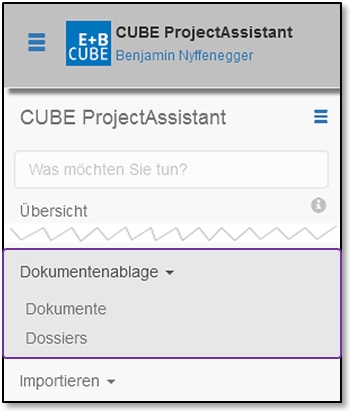
\includegraphics[width=1\linewidth]{../chapters/11_Dokumentenablage/pictures/11_Menu_Dokumentenablage.jpg}
  \end{center}
  \vspace{-20pt}
  \caption{Utilisation du classement des documents}
  \vspace{-10pt}
\end{wrapfigure}

Choisissez l'élément 'Classement des documents' dans le menu à gauche. Les sous-éléments 'Documents' et 'Dossiers' apparaissent.

\vspace{\baselineskip}

Le fonction de classement des documents est utilisée pour gérer et modifier les documents. Quand des documents ou leurs métadonnées sont modifiés, ils reçoivent un nouveau numéro de version dans CUBE PA. Les fonction d'extraction et de réintroduction de documents assurent qu'un document ne peut être modifié que par un seul utilisateur à la fois. D'autre part, l'attribution de versions aux documents assure que tous les participants au projet peuvent faire référence à des versions de documents uniques. 

\vspace{1cm}  

Les documents saisis ou chargés peuvent être classés dans des dossiers, qui peuvent ensuite être facilement téléchargés. Pour cette raison, la création et la gestion de dossiers sont décrites en premier dans ce chapitre.

\vspace{\baselineskip}

La gestion de documents est ensuite expliquée dans les détails.

\subsection{Dossiers}
\label{bkm:Ref442544219}\subsubsection{Créer des dossiers}

Un dossier est un ensemble de documents associés. Un exemple classique est un dossier d'approbation des plans ou un avant-projet. Les dossiers permettent de grouper plusieurs documents chargés, dans le but qu'ils puissent ensuite être téléchargés ensemble en tant qu'archive ZIP. 

\begin{figure}[H]
\center{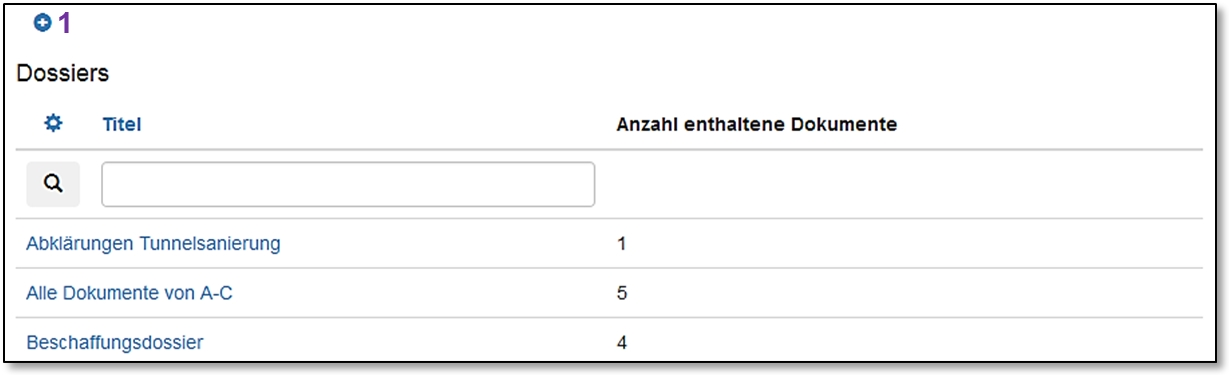
\includegraphics[width=1\linewidth]{../chapters/11_Dokumentenablage/pictures/11-1-1_UebersichtDossiers.jpg}}
\caption{Créer un nouveau dossier}
% \label{fig:speciation}
\end{figure}

Pour créer un nouveau dossier, sélectionnez l'élément de menu 'Classement des documents' et ensuite le sous-élément 'Dossiers'. Cliquez ensuite sur le symbole plus (ajouter) 
\includegraphics[height=12pt]{/Icons/Plussymbol.jpg} \col{(1)}.

\vspace{\baselineskip}

Le masque de saisie pour un dossier est ouvert :

\begin{figure}[H]
\center{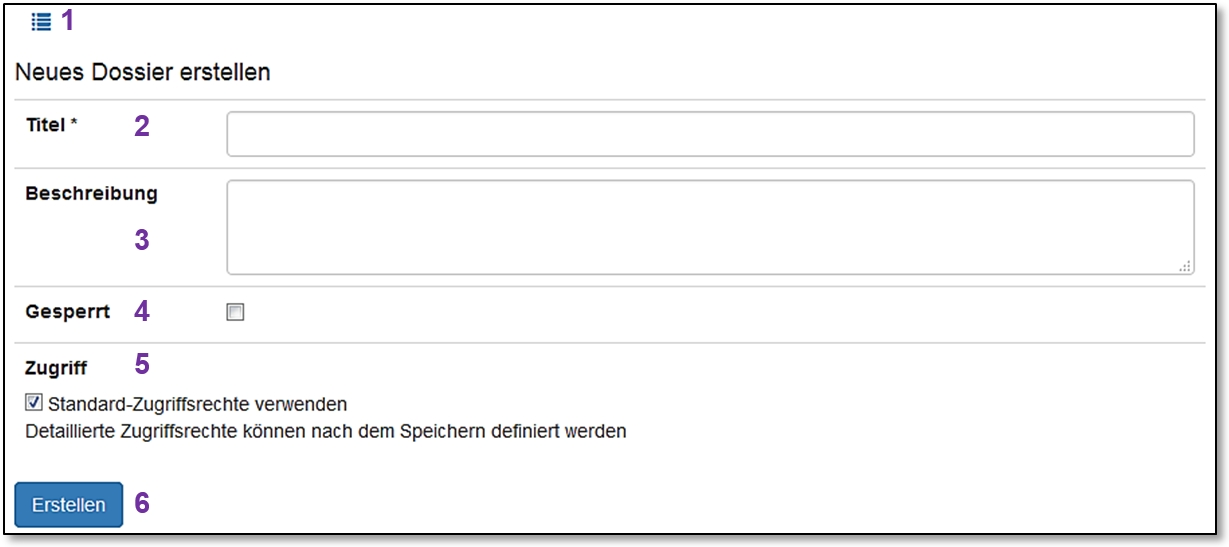
\includegraphics[width=1\linewidth]{../chapters/11_Dokumentenablage/pictures/11-1-1_DossierEingabemaske.jpg}}
\caption{Masque de saisie pour un nouveau dossier}
% \label{fig:speciation}
\end{figure}

Saisissez un titre significatif \col{(2)} pour le nouveau dossier. Comme plusieurs dossiers peuvent aborder le même sujet, il est recommandé d'indiquer la date dans le titre, comme par exemple 'Étude de faisabilité XY. Août 2015'. Il est également recommandé de vérifier, avant de créer un nouveau dossier, si un dossier avec un titre similaire existe déjà. Si tel est le cas, le même titre exactement devrait être utilisé, par exemple 'Étude de faisabilité XY. Août 2015' et 'Étude de faisabilité XY. Décembre 2015'. Une description détaillée \col{(3)} peut être ajoutée si nécessaire. Les dossiers peuvent être verrouillés contre les modifications. Si cette fonction est activée, l'ajout et le retrait des documents du dossier n'est pas possible. Pour ce faire, sélectionnez l'option 'Verrouillé' \col{(4)} en cochant la case correspondante. Le dossier ne sera plus disponible pour sélection dans le menu déroulant des documents. En cas de besoin, les dossiers peuvent être protégés par des droits d'accès. Si des droits d'accès spéciaux ne sont pas nécessaires, gardez la case 'Utiliser les droits d'accès par défaut' sous 'Accès' \col{(5)} cochée. Si le dossier ne doit être accessible qu'à certains groupes/utilisateurs, décochez la case. Vous pouvez définir plus tard quel(s) utilisateur(s) ou groupe(s) peuvent accéder au dossier. Pour plus d'informations sur les droits d'accès, voir chapitre \ref{bkm:Ref442273510}. \newline


Quand toutes les informations désirées ont été saisies, créez le dossier en cliquant sur le bouton 'Créer' \col{(6)}. Pour retourner à l'aperçu/liste de tous les documents, cliquez sur le symbole de liste 
\includegraphics[height=12pt]{/Icons/Listensymbol_zurueck.jpg} \col{(1)}.

\vspace{\baselineskip}

Quand un dossier est créé avec le bouton 'Créer', la vue d'ensemble suivante s'affiche :

\begin{figure}[H]
\center{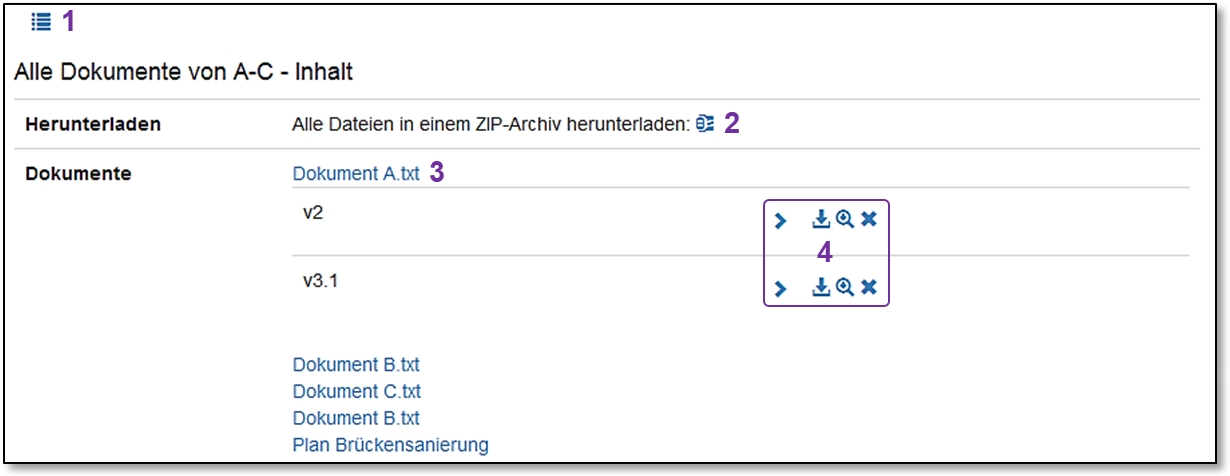
\includegraphics[width=1\linewidth]{../chapters/11_Dokumentenablage/pictures/11-1-1_UebersichtEinesDossiers.jpg}}
\caption{Vue d'ensemble du dossier}
% \label{fig:speciation}
\end{figure}

La saisie du dossier est maintenant visible. Cliquez sur le symbole ZIP 
\includegraphics[height=12pt]{/Icons/ZIPSymbol.jpg} \col{(2)} pour télécharger les documents contenus dans le dossier. Cliquez sur le titre d'un document en bleu \col{(3)} pour afficher les options (vous trouverez les explications relatives aux options plus bas). Les versions principales ou secondaires du document qui sont associées au dossier sont indiquées. Cliquez à nouveau sur le titre du document en bleu pour cacher les options.

Cliquez sur le symbole de liste 
\includegraphics[height=12pt]{/Icons/Listensymbol_zurueck.jpg} \col{(1)} pour retourner à l'aperçu/liste de tous les documents.

\vspace{\baselineskip}

Le classement des documents dans un dossier se fait dans la rubrique 'Documents' (Choisir l'élément 'Classement des documents' dans le menu à gauche puis le sous-élément 'Documents'). Pour ajouter des documents à un dossier, les documents doivent d'abord être chargés (voir chapitre \ref{bkm:Ref442769978}).

\subsubsection{Afficher et modifier un dossier}

Les options suivantes sont disponibles dans l'aperçu des dossiers :

\begin{figure}[H]
\center{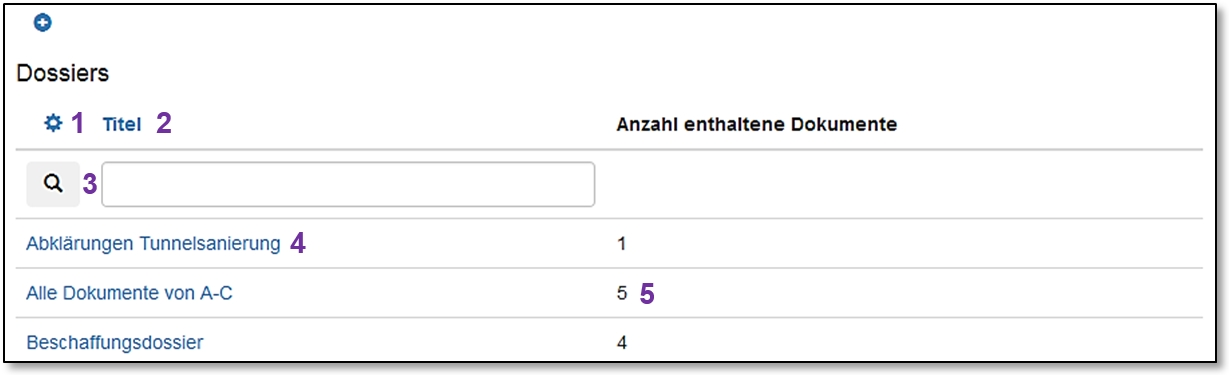
\includegraphics[width=1\linewidth]{../chapters/11_Dokumentenablage/pictures/11-1-2_UebersichtAllerDossiers.jpg}}
\caption{Aperçu de tous les dossiers}
% \label{fig:speciation}
\end{figure}

Vous pouvez afficher et masquer des colonnes en utilisant le symbole de configuration 
\includegraphics[height=12pt]{/Icons/SpaltenEinst.jpg} \col{(1)} (Ceci n'a pas d'effet dans l'aperçu des dossiers puisqu'il n'y a qu'une seule colonne). Cliquez sur 'Titre' \col{(2)} pour trier les dossiers par ordre alphabétique de A à Z. Cliquez à nouveau pour les trier par ordre alphabétique de Z à A.

\vspace{\baselineskip}

\textbf{Recherche :} Vous pouvez chercher un dossier dans l'aperçu. Sans utiliser un caractère de remplacement (*), vous pouvez directement saisir un mot clé et cliquer le symbole de loupe 
\includegraphics[height=12pt]{/Icons/Lupe_kl.jpg} \col{(3)} ou appuyer sur la touche Entrée. Tous les documents contenant le mot clé seront affichés. \newline

Cliquez sur le titre du dossier \col{(4)} pour aller directement à l'aperçu détaillé et au mode de modification du dossier. Dans l'aperçu détaillé vous pouvez également voir combien de documents contient le dossier \col{(5)}. La suppression de dossiers n'est pas possible pour le moment. \newline

Si vous ouvrez un dossier en cliquant sur son titre \col{(4)}, vous pouvez aussi voir tous les documents qu'il contient :

\begin{figure}[H]
\center{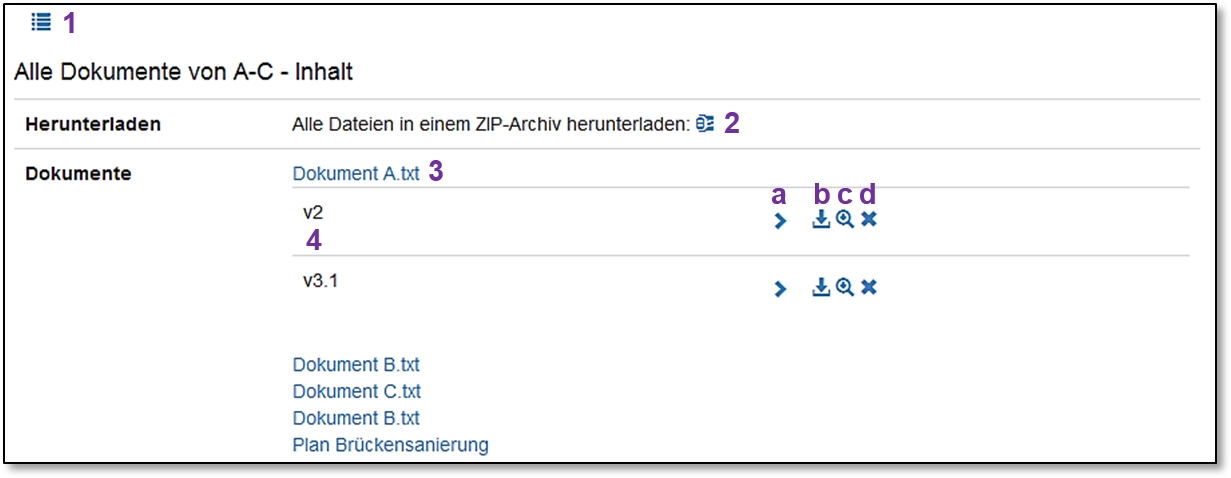
\includegraphics[width=1\linewidth]{../chapters/11_Dokumentenablage/pictures/11-1-2_DetailsEinesDossiers.jpg}}
\caption{Aperçu détaillé d'un dossier}
% \label{fig:speciation}
\end{figure}

Cliquez sur le symbole de liste 
\includegraphics[height=12pt]{/Icons/Listensymbol_zurueck.jpg} \col{(1)} pour retourner à l'aperçu de tous les dossiers. Vous pouvez télécharger tous les documents contenus dans le dossier en cliquant sur le symbole ZIP 
\includegraphics[height=12pt]{/Icons/ZIPSymbol.jpg} \col{(2)}. Une fenêtre de dialogue apparaît dans laquelle vous pouvez choisir si vous voulez sauvegarder l'archive ZIP sur votre ordinateur ou simplement l'ouvrir. La fenêtre dépend du navigateur que vous utilisez. \newline

Vous trouverez aussi une liste de tous les documents que contient le dossier. Cliquez sur le titre du document en bleu \col{(3)} pour afficher plus d'options. La version du document associée au dossier est indiquée \col{(4)}. \newline

Les options suivantes sont disponibles :
Avec le symbole de croix 
\includegraphics[height=12pt]{/Icons/blKreuzchen.jpg} \col{(d)} vous pouvez supprimer une version spécifique d'un document associé au dossier. Vous devez ensuite confirmer l'avertissement de sécurité.

\begin{figure}[H]
\center{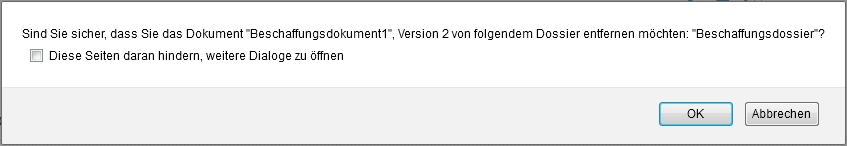
\includegraphics[width=.8\linewidth]{../chapters/11_Dokumentenablage/pictures/11-1-2_DokLoeschen_Meldung.jpg}}
% \caption{Detailansicht des Dossiers}
% \label{fig:speciation}
\end{figure}

Le symbole de loupe 
\includegraphics[height=12pt]{/Icons/Lupe.jpg} \col{(c)} vous dirige vers la saisie du document. Vous pouvez modifier la saisie du document, charger une nouvelle version du document, etc. Pour plus de détails sur le classement des documents, voir chapitre \ref{bkm:Ref442273482}. Le symbole de téléchargement 
\includegraphics[height=12pt]{/Icons/Download.jpg} \col{(b)} vous permet de télécharger une version spécifique du document (c'est-à-dire pas le dossier en entier). Selon le type de document, vous pouvez prévisualiser un document spécifique en ligne. Si cette option est disponible, une flèche orientée vers la droite 
\includegraphics[height=12pt]{/Icons/Pfeil_rechts.jpg} \col{(a)} est visible. Cliquez sur la flèche pour ouvrir la prévisualisation dans une petite fenêtre. Cliquez sur la flèche orientée maintenant vers le bas pour fermer la prévisualisation :


\begin{figure}[H]
\center{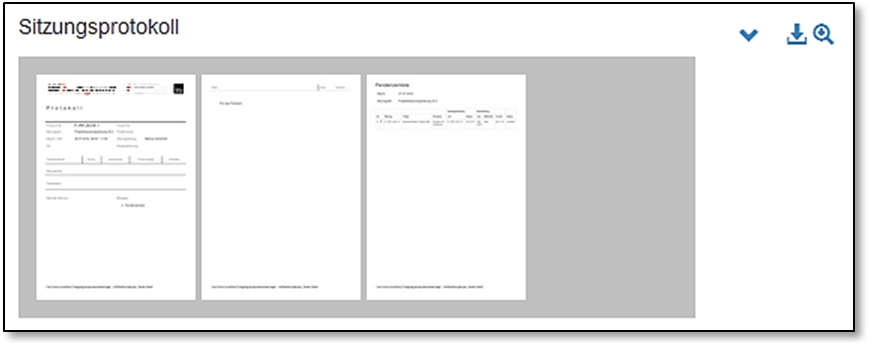
\includegraphics[width=0.75\linewidth]{../chapters/11_Dokumentenablage/pictures/11-1-2_Vorschau.jpg}}
\caption{Prévisualisation d'un document}
% \label{fig:speciation}
\end{figure}

\pagebreak

Cliquez sur une des pages de la prévisualisation pour ouvrir une visualisation détaillée de cette page :

\vspace{\baselineskip}

\begin{wrapfigure}[12]{r}{9cm}   % [x] Wie manche Zeile soll sich um die Grafik "brechen"
  \vspace{-30pt}      % Grundwert war 20; mit 30 schön oben beim Text ausgerichtet
  \begin{center}
    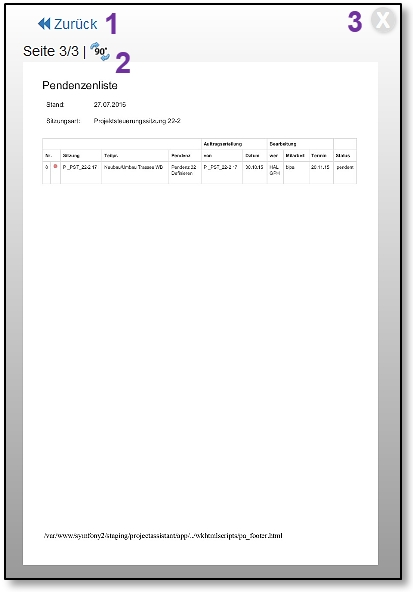
\includegraphics[height=110mm]{../chapters/11_Dokumentenablage/pictures/11-1-2_VorschauDetails.jpg}
  \end{center}
  \vspace{-20pt}
  \caption{Visualisation détaillée d'une page}
  \vspace{-10pt}
\end{wrapfigure}
En haut à gauche se trouve la navigation. Vous pouvez voir combien de pages contient le document et naviguer parmi les pages du document en cliquant les boutons 'Précédent' et 'Suivant' \col{(1)}. En cas de besoin (par exemple pour une carte ou un plan), vous pouvez tourner la page avec le symbole '90°' - cliquez une deuxième fois pour tourner la page de 90° supplémentaires, etc. Pour fermer la visualisation, cliquez sur le bouton 'X' \col{(3)}.

\vspace{5cm}

\subsubsection{Gérer les droits d'accès aux dossier}
\label{bkm:Ref442273510}
Pour chaque dossier, vous pouvez décider qui peut le lire, modifier, et/ou supprimer (la suppression de dossiers n'est pas disponible pour le moment). Vous pouvez attribuer les droits d'accès pour un ou plusieurs groupe(s) ou utilisateur(s). La procédure est décrite au chapitre \ref{bkm:Ref442869495} et est similaire à l'attribution de droits d'accès pour les documents.

\pagebreak
\subsection{Documents}
\label{bkm:Ref442273482}

\subsubsection{Aperçu des documents (Recherche de documents)}
\label{bkm:Ref443047823}

Choisissez l'élément 'Classement des documents' dans le menu à gauche puis le sous-élément 'Documents'. Une liste des documents saisis/chargés est affichée dans l'aperçu des documents.

\begin{figure}[H]
\center{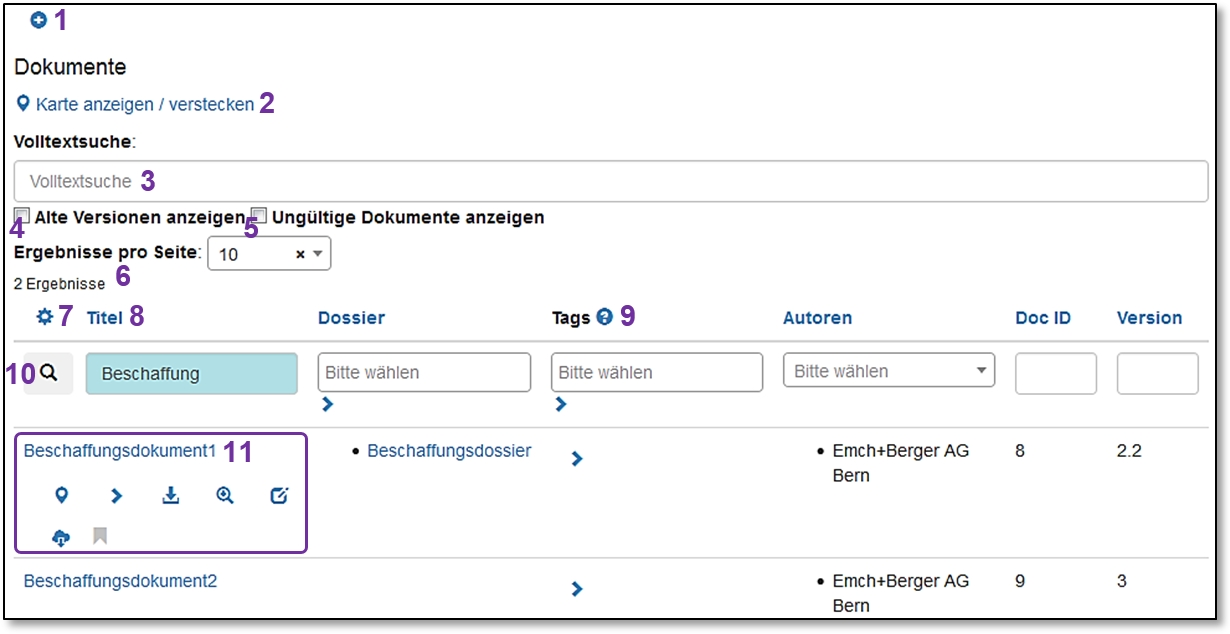
\includegraphics[width=1\linewidth]{../chapters/11_Dokumentenablage/pictures/11-2-1_DokumentenUebersicht.jpg}}
\caption{Aperçu des documents}
% \label{fig:speciation}
\end{figure}

Pour ajouter des nouveaux documents, cliquez sur le symbole plus (ajouter) 
\includegraphics[height=12pt]{/Icons/Plussymbol.jpg} \col{(1)}. Pour plus d'informations, voir chapitre \ref{bkm:Ref442770648}. 'Afficher / masquer carte' \col{(2)} vous permet d'afficher ou de masque une carte Google Maps. La recherche plein texte \col{(3)} permet de chercher les saisies en fonction de mots-clé. Après avoir saisi un mot-clé, cliquez sur le symbole de loupe 
\includegraphics[height=12pt]{/Icons/Lupe_kl.jpg} \col{(9)} ou appuyez sur la touche Entrée. Plusieurs mots-clé peuvent être saisis. Si vous cherchez un groupe de mots spécifique, écrivez-le entre guillemets. Avec la recherche plein texte, les titres de documents et de dossiers, les tags (étiquettes), et si techniquement possible, le contenu des documents sont cherchés. Pour inclure des anciennes versions et/ou des documents non valables dans la recherche, cochez la case 'Inclure anciennes versions' \col{(4)} et/ou la case 'Afficher les documents non valables' \col{(5)}. Le symbole de configuration 
\includegraphics[height=12pt]{/Icons/SpaltenEinst.jpg} \col{(6)} vous permet de masquer les colonnes non utilisées. Après avoir choisi les colonnes désirées, cliquez 'Actualiser' et l'aperçu des documents sera mis à jour. \newline
En plus de la recherche plein texte, vous pouvez effectuer des recherches par colonne \col{(7)}, ou bien choisir à l'aide des menus déroulants quels documents vous voulez afficher. Cliquez sur les en-têtes en bleu pour trier les documents par ordre alphabétique de A à Z. Cliquez à nouveau pour les trier par ordre alphabétique de Z à A. \newline
Les documents chargés peuvent être étiquetés par le moyen de tags \col{(8)}. Pour plus d'informations sur les tags, voir chapitre \ref{bkm:Ref442275849}.
Quand vous cliquez sur une saisie de données dans la liste \col{(10)} (dans la colonne Titre, texte en bleu), des options s'affichent. Les options sont expliquées plus bas.

\subsubsection{Ajouter un nouveau document}
\label{bkm:Ref442863508}\label{bkm:Ref442787515}\label{bkm:Ref442778397}\label{bkm:Ref442770648}\label{bkm:Ref442769978}

\begin{figure}[H]
\center{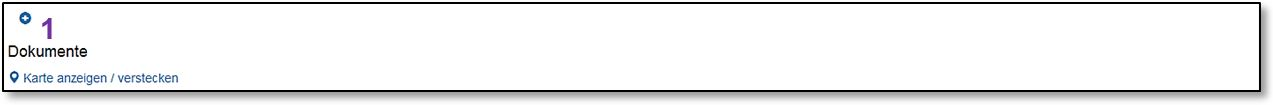
\includegraphics[width=1\linewidth]{1122_DokumenteHochladen.jpg}}
% \caption{Neues Dokument hochladen}
% \label{fig:speciation}
\end{figure}

Cliquez sur le symbole plus (ajouter) 
\includegraphics[height=12pt]{/Icons/Plussymbol.jpg} \col{(1)}. Le masque de saisie pour un nouveau document s'affiche :

\begin{figure}[H]
\center{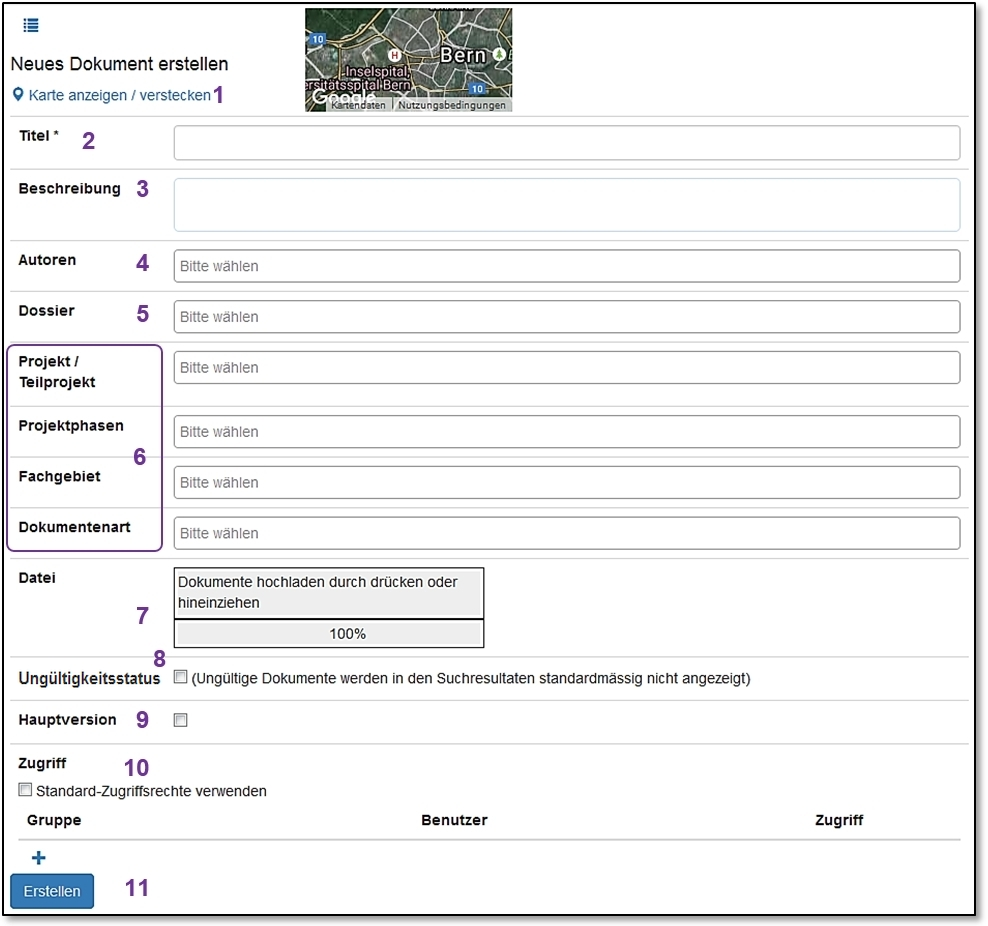
\includegraphics[width=1\linewidth]{../chapters/11_Dokumentenablage/pictures/11-2-2_NeuesDokuErstellen.jpg}}
\caption{Masque de saisie pour un nouveau document}
% \label{fig:speciation}
\end{figure}

Cliquez sur le lien 'Afficher / masquer carte' \col{(1)}, pour afficher Google Maps, ou pour passer à un affichage plus grand. Pour plus d'informations concernant l'association de documents à Google Maps, voir chapitre \ref{bkm:Ref442545553}. \newline

Le seul champ de saisie obligatoire pour l'ajout d'un document est le titre \col{(2)}. Dans la description \col{(3)}, des notes supplémentaires peuvent être saisies. Sous 'Auteurs' \col{(4)}, vous pouvez choisir le(s) auteur(s) par l'intermédiaire d'un menu déroulant. L'auteur doit être saisi au préalable. Si un auteur n'est pas sur la liste, il peut être ajouté par l'administrateur. Pour classer un document dans un dossier (voir chapitre \ref{bkm:Ref442544219}), choisissez le dossier correspondant dans le menu déroulant \col{(5)} (le dossier doit déjà exister). Un document peut être classé dans plusieurs dossiers. Cliquez à nouveau sur le menu déroulant pour choisir plus de dossiers pour le document. Des 'tags' (étiquettes) \col{(6)} peuvent être définis et attribués à un document. Ceci permet d'effectuer des recherches de tags spécifiques pour trouver des documents de projets, phases de projet, domaines d'expertise, ou types de documents spécifiques. Les thèmes de tags (par exemple domaine d'expertise) et les tags individuels (par exemple passages à niveau, éclairage, exploitation, etc.) ne peuvent être définis ou ajoutés que par l'administrateur. Si un tag manque, veuillez contacter l'administrateur.

Sous 'Fichier' \col{(7)}, cliquez dans le rectangle gris pour charger un fichier. Une fenêtre s'affiche, dans laquelle vous pouvez naviguer pour choisir le document désiré. Alternativement, vous pouvez charger un ou plusieurs fichiers en glissant-déposant dans le rectangle gris.

\begin{figure}[H]
\center{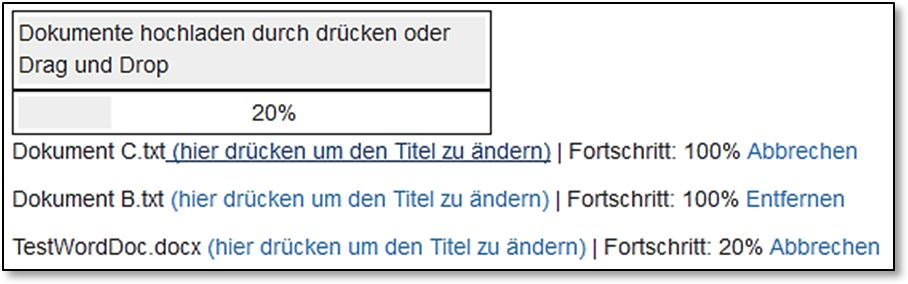
\includegraphics[width=0.75\linewidth]{1122_MehrereDokumenteHochladen.jpg}}
\caption{Charger plusieurs documents}
% \label{fig:speciation}
\end{figure}

Le progrès de chargement des fichiers individuels est affiché. Vous pouvez enlever des fichiers en cliquant 'Enlever' ou arrêter le chargement en cliquant 'Annuler'. Le premier fichier chargé est renommé avec le titre du document. Les autres fichiers ne sont pas renommés. Tous les titres des fichiers peuvent être modifiés en cliquant '(veuillez appuyer ici pour changer le titre)' :

\begin{figure}[H]
\center{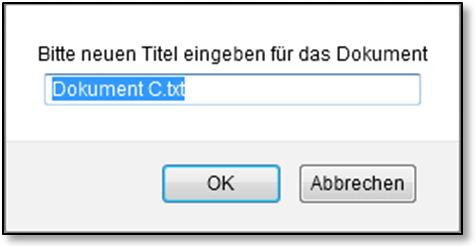
\includegraphics[width=0.4\linewidth]{1122_DokumentenTitelAendern.jpg}}
\caption{Changement de titre}
% \label{fig:speciation}
\end{figure}

Pour chaque document chargé une saisie séparée, mais avec les mêmes données (description, auteurs, dossiers, etc.) est créée. Ceci permet d'économiser du temps, surtout pour la création d'un dossier avec plusieurs documents ayant la même description, auteurs, etc.

Si un document n'est plus valable, il peut être exclu des résultats de recherche en cochant la case 'Non valable' \col{(8)}. Cette fonction n'est pas à confondre avec les versions de documents, qui font que les anciennes versions d'un document ne soient par défaut pas affichées dans les résultats de recherche.\newline

Vous pouvez indiquer si un fichier chargé constitue une version principale (V1, V2, V3, etc.) ou une version secondaire (V3.1, V3.2, etc.) d'un document. Si le fichier chargé est une version principale, cochez la case 'Version principale' \col{(9)}.

Vous pouvez attribuer les droits d'accès par défaut \col{(10)} à un document ou autoriser l'accès à certaines personnes seulement. Les droits d'accès peuvent être adaptés et élargis à tout moment plus tard dans le mode de modification. Le chapitre \ref{bkm:Ref442869495} offre plus d'informations sur la gestion des droits d'accès.

Quand toutes les informations nécessaires sont saisies, le document est chargé en cliquant le bouton 'Créer' \col{(11)} et les saisies sont enregistrées. \newline

\textbf{Remarque :} Un document peut être uniquement remplacé par un seul autre document. Si vous essayez de déposer plusieurs fichiers dans la fenêtre de chargement, le message d'erreur suivant s'affiche :

\begin{figure}[H]
\center{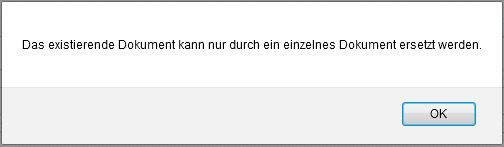
\includegraphics[width=0.75\linewidth]{1122_FehlerDokumentErsetzen.jpg}}
\caption{Message d'erreur pour le chargement de plusieurs fichiers}
% \label{fig:speciation}
\end{figure}

\textbf{Note :} Si uniquement les métadonnées d'un document sont modifiées et enregistrées, une nouvelle version du document ne sera pas créée. Les changements dans les métadonnées apparaîtront par contre dans l'historique du document. Similairement, si le même fichier est chargé (dans lequel aucun changement n'a été effectué) ou bien si un document a été extrait puis réintroduit sans aucune modification, CUBE PA ne crée pas une nouvelle version du document. Le message suivant s'affiche :

\begin{figure}[H]
\center{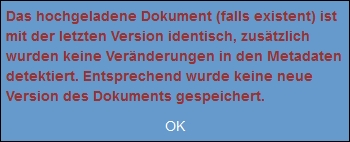
\includegraphics[width=0.5\linewidth]{../chapters/11_Dokumentenablage/pictures/11-2-2_Meldung_gleicheDatei.jpg}}
\caption{Message : Nouvelle version de document non créée}
% \label{fig:speciation}
\end{figure}

Pour pouvoir continuer à travailler, vous devez d'abord cliquer sur 'OK' dans le dialogue ci-dessus.

\subsubsection{Documents avec lien Google Maps}
\label{bkm:Ref442545553}
Les documents peuvent être associés à Google Maps. De cette manière, les documents liés à un lieu spécifique peuvent être repérés, modifiés ou téléchargés. \\
Passez au mode de modification du document désiré avec le symbole de modification 
\includegraphics[height=12pt]{/Icons/Bearbeiten.jpg} (Dans le mode d'affichage, les liens Google Maps peuvent être visualisés mais vous ne pouvez pas créer, ajouter ou supprimer un lien).

% \vspace{\baselineskip}
\vspace{2mm}

\begin{wrapfigure}[15]{l}{6.5cm}
\vspace{-15pt}
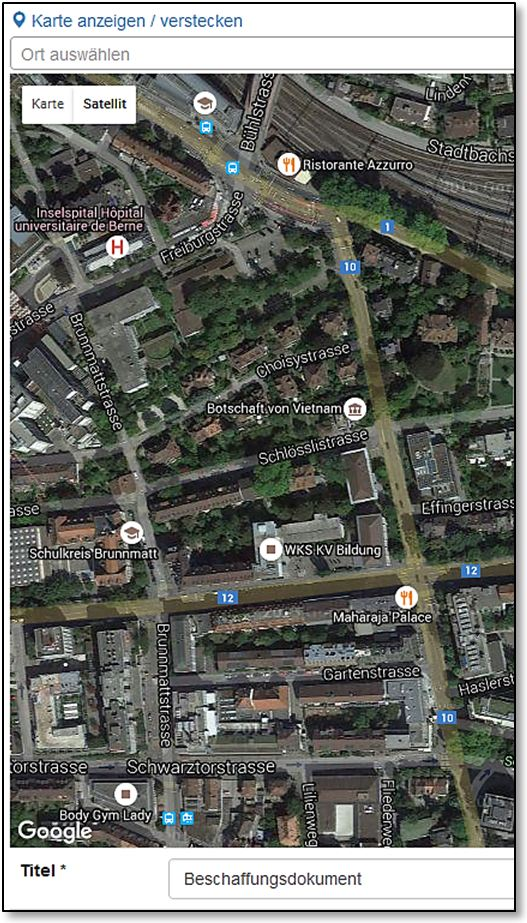
\includegraphics[height=110mm]{1123_GoogleMap.jpg}
% \caption{Status ändern}
\end{wrapfigure}

Pour lier un document à un lieu sur la carte, double-cliquez sur l'objet/le lieu désiré sur la carte. Vous pouvez également choisir un lieu prédéfini. Pour ce faire, cliquez sur le champ de saisie 'Choisir lieu' au-dessus de la carte et choisissez le lieu désiré.

\vspace{4mm}

\hspace{15mm} 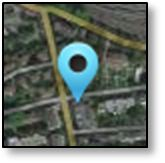
\includegraphics[height=20mm]{1123_GoogleMapNadel.jpg}

Le repère ci-dessus s'affiche. Vous pouvez ensuite déplacer ce repère vers un autre lieu par 'drag \& drop' (glisser-déposer).

\hspace{15mm} 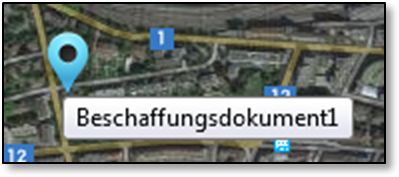
\includegraphics[height=20mm]{1123_GoogleMapText.jpg}

Déplacez le curseur au-dessus du repère pour voir quel ou quels documents sont liés à ce lieu. \\

Répétez les étapes ci-dessus pour ajouter plus de liens Google Maps. Pour supprimer un lien spécifique, cliquez sur le repère avec le bouton droit de la souris. Le dialogue suivant s'affiche, et vous demande de confirmer la suppression des coordonnées : 

\begin{figure}[H]
\center{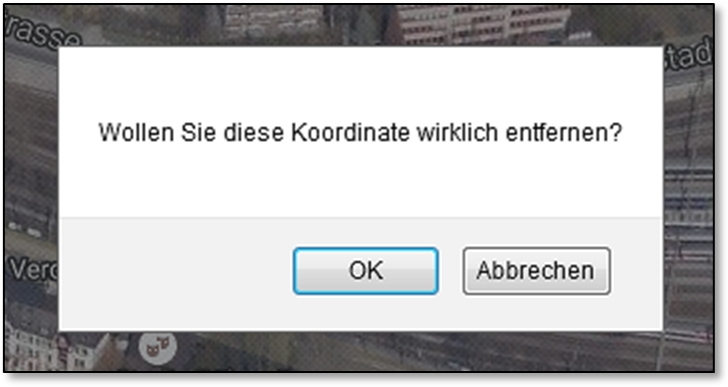
\includegraphics[width=0.5\linewidth]{../chapters/11_Dokumentenablage/pictures/11-2-3_DialogLoeschen.jpg}}
\caption{Supprimer un lien}
% \label{fig:speciation}
\end{figure}

\vspace{\baselineskip}

\textbf{Utiliser Google Maps dans CUBE PA :}

L'utilisation de Google Maps dans CUBE PA est identique à l'utilisation de Google Maps dans un navigateur. Cliquez et maintenez appuyé le bouton de la souris pour déplacer la carte. Si votre souris dispose d'une molette de défilement, utilisez cette dernière pour zoomer sur la carte. (Les touches de fonction comme Shift, Ctrl et Alt ne fonctionnent pas dans l'utilisation de la carte).

\vspace{\baselineskip}

\textbf{Rechercher un lieu :} 

\begin{figure}[H]
\center{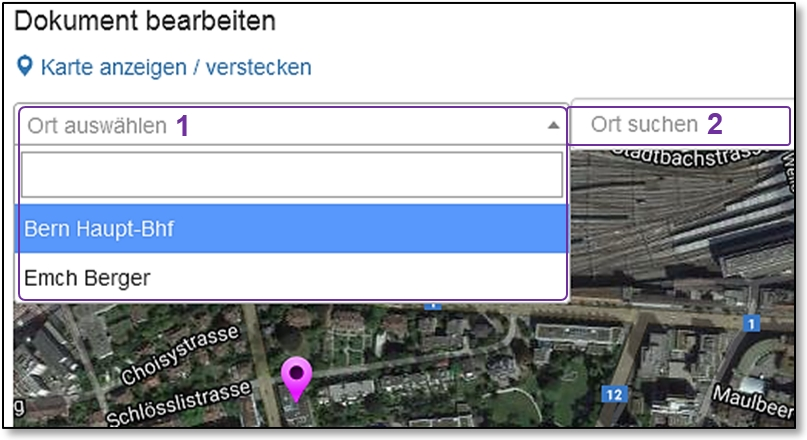
\includegraphics[width=0.6\linewidth]{../chapters/11_Dokumentenablage/pictures/11-2-3_GeographischSuchen.jpg}}
\caption{Rechercher un lien}
% \label{fig:speciation}
\end{figure}

Quand Google Maps est affiché dans l'aperçu des documents (cliquez sur 'Afficher / masquer la carte'), tous les documents avec un lien Google Maps sont affichés. Vous pouvez choisir un lieu du menu déroulant \col{(1)} ou chercher un lieu en saisissant l'information dans le champ \col{(2)} et en appuyant la touche Entrée. Google Maps naviguera au lieu désiré et affichera tous les documents qui y sont associés. Si vous avez filtré la liste de documents dans l'aperçu des documents, seuls les documents filtrés apparaîtront sur la carte. \newline

\textbf{Filtrer les documents selon la zone géographique :} \\

\begin{wrapfigure}[9]{r}{7cm}
  \vspace{-35pt}
  \begin{center}
    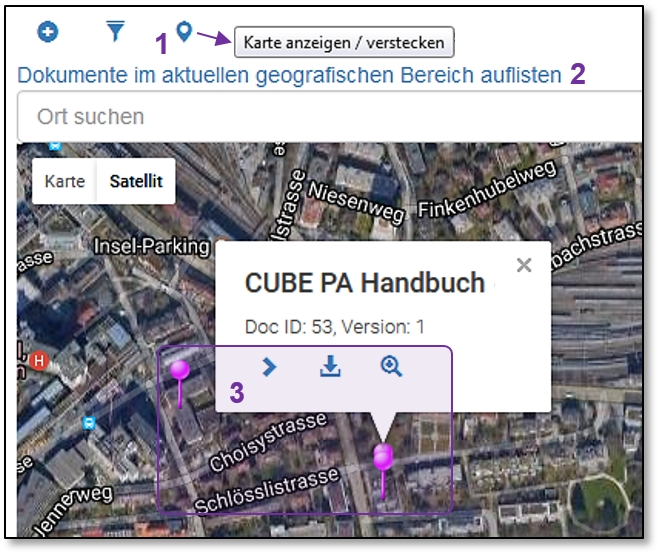
\includegraphics[height=55mm]{../chapters/11_Dokumentenablage/pictures/11-2-3_GeoBereichFilter.jpg}
  \end{center}
  \vspace{-20pt}
  % \caption{Geografische Bereiche filtern}
  \vspace{-10pt}
\end{wrapfigure}
Vous avez la possibilité de filtrer les documents qui sont dans la même zone géographique ou qui ont des coordonnées proches. Pour ce faire, cliquez sur 'Afficher / masquer carte' \col{(1)} pour afficher Google Maps. La fonction 'Afficher les documents dans la zone géographique actuelle' \col{(2)} s'affiche. Cliquez dessus pour définir un filtre géographique :

\vspace{1cm} 

\begin{wrapfigure}[12]{r}{8cm}
  \vspace{-25pt} 
  \begin{center}
    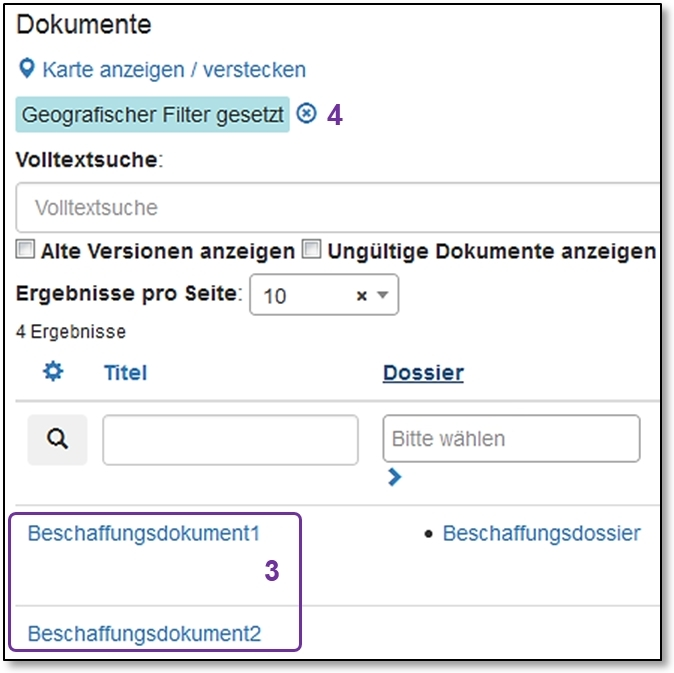
\includegraphics[height=70mm]{../chapters/11_Dokumentenablage/pictures/11-2-3_GeoBereichResult.jpg}
  \end{center}
  \vspace{-20pt}
  % \caption{Dokumenten in einem gemeinsamen geografischen Bereich}
  \vspace{-10pt}
\end{wrapfigure}

'Filtre géographique défini' s'affiche au dessus des champs de recherche / filtrage. Seuls les documents ayant des coordonnées géographiques proches s'affichent. Dans cet exemple, deux document sont listés. Ce sont les deux documents indiqués par des repères sur la carte dans la prise d'écran précédente \col{(3)}. Il s'agit des deux documents des résultats de recherche. Pour enlever le filtre géographique, cliquez sur la petite croix près de 'Filtre géographique défini' \col{(4)}. Cliquez ensuite sur le symbole de loupe 
\includegraphics[height=12pt]{/Icons/Lupe.jpg} pour afficher la liste de résultats non filtrée.

\subsubsection{Travailler avec les documents chargés}
\label{bkm:Ref442801819}

\begin{figure}[H]
\center{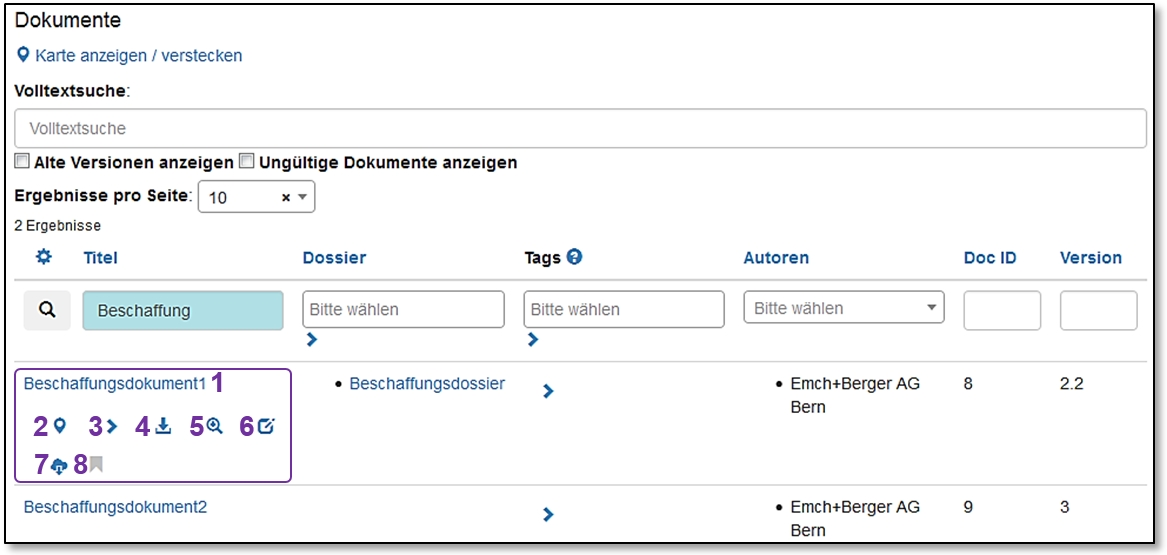
\includegraphics[width=1\linewidth]{../chapters/11_Dokumentenablage/pictures/11-2-4_FunktionenHochgDateien.jpg}}
\caption{Options pour les documents chargés}
% \label{fig:speciation}
\end{figure}

Vous pouvez chercher des documents dans l'aperçu des documents (voir chapitre \ref{bkm:Ref443047823}). Cliquez sur le titre du document désiré (police bleue) \col{(1)} pour visualiser les différentes options. Cliquez sur le titre à nouveau pour masquer les options.

Si le document est associé à Google Maps, cliquez sur le symbole de repère 
\includegraphics[height=12pt]{/Icons/Nadelsymbol.jpg} \col{(2)} pour naviguer directement au lieu du document sur la carte. Le symbole de repère est uniquement visible si un lien à Google Maps existe (voir chapitre \ref{bkm:Ref442545553}). La fenêtre suivante s'ouvre :

\begin{figure}[H]
\center{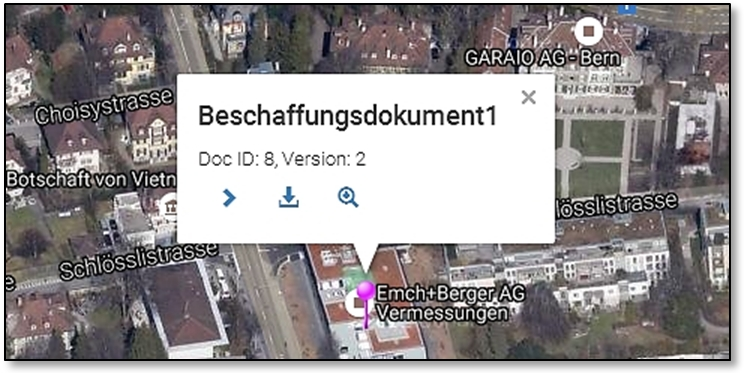
\includegraphics[width=0.5\linewidth]{../chapters/11_Dokumentenablage/pictures/11-2-4_DokAufGoogleMaps.jpg}}
% \caption{Das Menü in CUBE PA}
% \label{fig:speciation}
\end{figure}

Depuis cette fenêtre, vous avez la possibilité d'ouvrir la prévisualisation du document, de télécharger le document, ou d'afficher la saisie du document. Cliquez sur la croix dans le coin supérieur droit de la fenêtre pour la fermer. \newline

Cliquez sur le symbole de flèche 
\includegraphics[height=12pt]{/Icons/Pfeil_rechts.jpg} \col{(3)} pour prévisualiser le document dans l'aperçu des documents, dans la mesure où le format du fichier est supporté. Cliquez sur la flèche 
\includegraphics[height=12pt]{/Icons/Pfeil_unten.jpg} à nouveau pour fermer la prévisualisation. Plus d'informations sur la prévisualisation sont données plus bas.\newline

Vous pouvez également directement télécharger le document \includegraphics[height=12pt]{/Icons/download.jpg} \col{(4)}, visualiser la saisie du document 
\includegraphics[height=12pt]{/Icons/Lupe.jpg} \col{(5)} ou modifier la saisie du document 
\includegraphics[height=12pt]{/Icons/Bearbeiten.jpg} \col{(6)}. \newline

Pour modifier un document en ligne, il doit être extrait avec le symbole 
\includegraphics[height=12pt]{/Icons/Auschecken.jpg} \col{(7)}. La procédure est décrite dans les détails au chapitre \ref{bkm:Ref442776572}. Cliquez sur le symbole de drapeau gris \includegraphics[height=12pt]{/Icons/DokuFlag_grau.jpg} \col{(8)} pour ajouter un document à vos favoris. Le symbole devient rouge et le document est ajouté à votre aperçu personnel (voir chapitre \ref{bkm:Ref132000001}). Cliquez à nouveau sur le symbole rouge \includegraphics[height=12pt]{/Icons/DokuFlag_rot.jpg} pour enlever le document de vos favoris. \newline

\pagebreak
\subsubsection{Visualiser la saisie d'un document}
\label{bkm:Ref443047930}

\begin{wrapfigure}[18]{l}{9.5cm}
\vspace{-15pt}
\includegraphics[height=105mm]{../chapters/11_Dokumentenablage/pictures/11-2-5_Dokumentenansicht.jpg}
% \caption{Status ändern}
\end{wrapfigure}

Quand vous cliquez sur le symbole de loupe \includegraphics[height=12pt]{/Icons/Lupe.jpg}, 
la saisie du document est ouverte en mode de visualisation. A côté du titre \col{(1)}, toutes les informations (par exemple auteur(s), tags ajoutés lors du chargement ou de la modification du document (voir \ref{bkm:Ref442778397}), etc.) sont affichées. Quand une information manque, le champ correspondant est soit vide soit non affiché. La version du document, l'horodatage, et l'utilisateur qui a modifié le document sont affichés en-dessous du titre \col{(2)}. \newline

Si le document est classé dans un dossier, vous pouvez ouvrir le dossier correspondant en cliquant sur le lien en bleu \textbf{\col{(3)}} dans le champ 'Dossier'. Sous 'Aperçu' \col{(4)}, une prévisualisation des premières pages du document est affichée en petit.

\vspace{\baselineskip}

Cliquez sur une des pages prévisualisées \col{(5)} pour ouvrir la page dans le mode de prévisualisation. Cliquez \includegraphics[height=11pt]{/Icons/Weiter.jpg} et \includegraphics[height=11pt]{/Icons/Zurueck.jpg} \col{(7)} pour naviguer les pages du document. Le nombre de pages \col{(8)} est affiché sous les boutons de navigation. Vous pouvez tourner les pages de 90° avec le symbole 90° \includegraphics[height=12pt]{/Icons/90Grad.jpg} \col{(9)}. Cliquez sur la croix grise \includegraphics[height=12pt]{/Icons/X_Button.jpg} \col{(6)} dans le coin droit supérieur de la prévisualisation pour la fermer.

\begin{figure}[H]
\center{\includegraphics[width=1\linewidth]{../chapters/11_Dokumentenablage/pictures/11-2-5_Dokumentenvorschau.jpg}}
\caption{Prévisualisation d'un document}
% \label{fig:speciation}
\end{figure}

Pour télécharger le document, cliquez le symbole de téléchargement \includegraphics[height=12pt]{/Icons/Download.jpg} ou le nom du fichier \col{(1)}. La fenêtre de téléchargement usuelle de votre navigateur s'affichera et vous pouvez choisir d'ouvrir ou de sauvegarder le document. 'Lien statique à la dernière version du fichier' \col{(2)} est un lien que vous pouvez envoyer par e-mail par exemple, tout en restant assuré que le destinataire sera toujours dirigé vers la dernière version du document. Dans le champ 'Extraire fichier' \includegraphics[height=12pt]{/Icons/Auschecken.jpg} \col{(3)}, la dernière version du document peut être extraite (voir chapitre \ref{bkm:Ref442780171}).

\begin{figure}[H]
\center{\includegraphics[width=1\linewidth]{1125_Dokumentenoptionen.jpg}}
\caption{Options pour documents chargés}
% \label{fig:speciation}
\end{figure}

Sous 'Historique', cliquez sur le symbole de flèche \includegraphics[height=12pt]{/Icons/Pfeil_rechts.jpg} \col{(4)} et les modifications du document s'affichent.

\begin{figure}[H]
\center{\includegraphics[width=1\linewidth]{1125_Aenderungshistorie.jpg}}
\caption{Visualisation de l'historique d'un document}
% \label{fig:speciation}
\end{figure}

Une liste avec les modifications s'affiche. Les modifications des données du document (par exemple, auteurs, tags) et les modifications du document lui-même (nouvelles versions) sont inclues dans la liste. Cliquez sur le symbole de téléchargement \includegraphics[height=12pt]{/Icons/Download.jpg} \col{(6)} pour télécharger une ancienne version du document ou sur le symbole de loupe \includegraphics[height=12pt]{/Icons/Lupe.jpg} \col{(5)} pour visualiser une ancienne version du document. \newline

\begin{wrapfigure}[7]{r}{6cm}
\vspace{-15pt}
\includegraphics[height=40mm]{1125_DokumentAeltereVersion.jpg}
% \caption{Status ändern}
\end{wrapfigure}

Si vous ouvrez une ancienne version d'un document, l'avertissement \textcolor{red}{'Cette version n'est pas la dernière version de ce document!'} apparaît dans l'aperçu de ce document. Si vous téléchargez le document dans le champ 'Fichier', vous n'accédez pas à la dernière version du document, mais à la version ancienne sélectionnée et affichée.

\begin{wrapfigure}[7]{r}{6cm}
% \vspace{-15pt}
\includegraphics[height=35mm]{1125_DokumentBearbeiten.jpg}
% \caption{Status ändern}
\end{wrapfigure}
Pour modifier les informations d'un document ou pour charger une nouvelle version d'un document, cliquez sur le symbole de modification en haut à gauche \includegraphics[height=12pt]{/Icons/Bearbeiten.jpg} \col{(1)}. Le symbole de liste \includegraphics[height=12pt]{/Icons/Listensymbol_zurueck.jpg} \col{(2)} vous permet de retourner à l'aperçu des documents. (Dans la visualisation d'une ancienne version d'un document, le symbole de modification n'est pas disponible. Vous pouvez cliquer sur le symbole de liste \includegraphics[height=12pt]{/Icons/Listensymbol_zurueck.jpg} pour retourner à l'aperçu des documents.)

\vspace{\baselineskip}

\textbf{Détails à propos de l'historique} \\
Toutes les modifications sont enregistrées dans l'historique. D'une part, l'historique enregistre quand un nouveau document (une version révisée) est chargé. D'autre part, les modifications des métadonnées sont aussi enregistrées dans l'historique, sans générer une nouvelle version du document (voir chapitre \ref{bkm:Ref442863508}).

\begin{figure}[H]
\center{\includegraphics[width=1\linewidth]{../chapters/11_Dokumentenablage/pictures/11-2-5_AenderungshistorieUebersicht.jpg}}
\caption{L'aperçu de l'historique d'un document}
% \label{fig:speciation}
\end{figure}

\col{(1)} Dans l'historique, la version du document actuellement ouverte dans le mode de visualisation est affichée avec en caractères gras. Vous pouvez également voir de quelle version du document il s'agit. Les saisies différentes sont séparées par des lignes \col{(2)}. Tous les changements sont enregistrés. Première saisie : Un nouveau fichier a été chargé et une description (métadonnée) a été ajoutée. Deuxième saisie : Le document a seulement été ajouté au dossier d'acquisition. Vous pouvez voir à quelle heure et par qui les modifications ont été effectuées. Pour ouvrir une prévisualisation de la dernière version ou d'une ancienne version du document, cliquez sur le symbole de flèche \includegraphics[height=12pt]{/Icons/Pfeil_rechts.jpg} \col{(3)}. Cliquez sur une des pages pour l'afficher en grand. Vous avez la possibilité de naviguer les pages du document ou de tourner les pages de 90°. Cliquez sur la croix \includegraphics[height=12pt]{/Icons/X_Button.jpg} en haut à droite pour fermer la prévisualisation en grand format. Cliquez sur le symbole de flèche (pointant vers le bas \includegraphics[height=12pt]{/Icons/Pfeil_unten.jpg}) pour fermer la petite prévisualisation.

Dans l'historique, vous pouvez télécharger la dernière version ou une ancienne version d'un document en cliquant sur le symbole de téléchargement \includegraphics[height=12pt]{/Icons/download.jpg} \col{(4)}. Utilisez le symbole de loupe \includegraphics[height=12pt]{/Icons/Lupe.jpg} \col{(5)} pour ouvrir la version correspondante (ancienne) du document en mode de visualisation. Vous avez aussi la possibilité de modifier les métadonnées d'une ancienne version. Pour ce faire, cliquez sur le symbole de modification \includegraphics[height=12pt]{/Icons/Bearbeiten.jpg} \col{(6)}. Avant de modifier, assurez-vous d'avoir ouvert la bonne version.

\vspace{\baselineskip}

\textbf{Remarque :} La modification d'anciennes versions de documents (métadonnées, droits d'accès) est uniquement possible en passant par l'historique, comme décrit ci-dessus.

\vspace{\baselineskip}

\textbf{Charger une nouvelle version d'un document}

\vspace{\baselineskip}

\begin{wrapfigure}[13]{r}{6cm}
\vspace{-35pt}
\includegraphics[height=100mm]{1125_DokumentBearbeitenFelder.jpg}
% \caption{Status ändern}
\end{wrapfigure}
Dans le mode de modification, vous pouvez compléter les informations d'un document (voir chapitre \ref{bkm:Ref442787515}). Pour charger une nouvelle version d'un document, cliquez sous 'Fichier' sur 'Recherche' \col{(1)} et choisissez le fichier désiré. En cas de besoin, d'autres saisies (métadonnées) peuvent être modifiées.

\vspace{\baselineskip}

Quand toutes les saisies nécessaires ont été faites, cliquez sur 'Accepter' \includegraphics[height=12pt]{/Icons/B_Uebernehmen.jpg} en bas à gauche pour charger le document et enregistrer les saisies. L'ancienne version (document et métadonnées) reste enregistrée et peut être accédée à tout moment dans l'historique du document.

\vspace{\baselineskip}
\vspace{\baselineskip}

\textbf{Remarque :} Si plusieurs versions d'un document sont classées dans un même dossier, seule la dernière version sera inclue dans le dossier (ceci se fait automatiquement). Ceci doit être spécialement pris en compte lors de chargement de nouvelles versions de documents. Si par exemple une nouvelle version d'un document ne doit plus être classée dans un certain dossier, la saisie du dossier doit être enlevée en chargeant le document (en cliquant sur l''X' dans le champ 'Dossier' \col{(2)}. De cette manière, les anciennes versions du document ne seront pas "écrasées" dans le dossier.

\begin{figure}[H]
\center{\includegraphics[width=1\linewidth]{1125_DokEintragLoeschen.jpg}}
\caption{Suppression de la saisie d'un dossier}
% \label{fig:speciation}
\end{figure}

\subsubsection{Gérer les droits d'accès aux documents}
\label{bkm:Ref442869495}

Vous pouvez choisir pour chaque document qui peut lire, modifier, et/ou supprimer le document (la suppression de documents est pour l'instant pas possible). Vous pouvez attribuer des droits d'accès pour un ou plusieurs groupes ou pour un ou plusieurs utilisateurs :

\begin{figure}[H]
\center{\includegraphics[width=1\linewidth]{1126_DokumentZugriffsrechte.jpg}}
\caption{Modifier un document - Attribuer des droits d'accès}
% \label{fig:speciation}
\end{figure}

Pour enlever les droits d'accès existants, cliquez sur le symbole de poubelle \includegraphics[height=12pt]{/Icons/Muelltonne.jpg} \col{(2)} puis confirmer l'avertissement qui s'affiche. \newline

Vous pouvez modifier les droits d'accès : Sélectionnez un groupe qui peut visualiser / modifier le document (le groupe doit déjà exister) ou sélectionnez une personne. Cliquez sur la petite flèche \includegraphics[height=12pt]{/Icons/Dropdown.jpg} \col{(3)} près de 'Veuillez choisir' ou du nom. Un menu déroulant vous affiche les groupes / personnes que vous pouvez choisir. Sous 'Accès' \col{(4)}, choisissez les droits du groupe / de la personne sélectionné(e) : lire / modifier / supprimer. Le symbole plus (ajouter) \includegraphics[height=12pt]{/Icons/Pluszeichen.jpg} \col{(5)} vous permet d'ajouter plus de groupes / personnes et de définir les droit d'accès comme décrit ci-dessus. \newline

Une fois les modifications nécessaires effectuées, cliquez 'Accepter' \col{(6)}. Cliquez sur le symbole de liste \col{(1)} pour retourner à l'aperçu des documents.

\subsubsection{Modifier documents en ligne / Extraire et réintroduire des documents}
\label{bkm:Ref442780171}\label{bkm:Ref442776572}

Pour modifier le contenu d'un document puis enregistrer une nouvelle version du document dans le classement des documents, suivez les étapes suivantes :

\begin{figure}[H]
\center{\includegraphics[width=.75\linewidth]{../chapters/11_Dokumentenablage/pictures/11-2-7_DokumentAusEinchecken.jpg}}
\caption{Fonctions dans l'aperçu des documents}
% \label{fig:speciation}
\end{figure}

Dans l'aperçu des documents, cliquez sur le titre en bleu du document désiré \col{(1)}. Les options s'affichent. Cliquez sur le symbole d'extraction \includegraphics[height=12pt]{/Icons/Auschecken.jpg} \col{(4)}. Alternativement, vous pouvez extraire le document dans le mode de visualisation du document (accessible par le symbole de loupe \includegraphics[height=12pt]{/Icons/Lupe.jpg} \col{(3)} dans l'aperçu des documents). Le document sera extrait, ouvert, et verrouillé contre les modifications par d'autres utilisateurs. Vous pouvez maintenant directement travailler dans le document.

\begin{wrapfigure}[5]{r}{6cm}
\vspace{-15pt}
\includegraphics[height=30mm]{1127_WordSpeichern.jpg}
% \caption{Status ändern}
\end{wrapfigure}
Pour arrêter la modification, enregistrez le document en cliquant le symbole correspondant dans le programme MS Office \col{(1)} (ici Office 2013 -- en haut à gauche) ou avec le raccourci 'Ctrl+S'. Le document mis à jour sera directement enregistré sur le serveur. Pour continuer à modifier le document ultérieurement, cliquez le symbole \includegraphics[height=12pt]{/Icons/Wolke_blauklein.jpg} \col{(2)} (ouvrir le document extrait) dans l'aperçu des document ou dans le mode de visualisation du document que vous voulez modifier.

\begin{figure}[H]
\center{\includegraphics[width=1\linewidth]{../chapters/11_Dokumentenablage/pictures/11-2-7_DokumentOeffnen.jpg}}
\caption{Ouvrir un document extrait}
% \label{fig:speciation}
\end{figure}

Une fois les modifications terminées, vous pouvez réintroduire le document en cliquant sur le symbole de réintroduction \includegraphics[height=12pt]{/Icons/Einchecken.jpg} \col{(3)} dans l'aperçu des documents ou dans le mode de visualisation du document. Le dernier document enregistré dans le serveur est fixé comme dernière version dans le classement des documents. Les symboles pour ouvrir un document extrait ou réintroduire un document extrait sont uniquement visibles pour les documents qui sont extraits.

\begin{figure}[H]
\center{\includegraphics[width=1\linewidth]{../chapters/11_Dokumentenablage/pictures/11-2-7_DokumentEinchecken.jpg}}
\caption{Réintroduire un document extrait}
% \label{fig:speciation}
\end{figure}

Comme alternative pour la modification de documents en ligne, vous pouvez aussi travailler 'offline'. Pour ce faire, il faut extraire le document comme décrit ci-dessus. Ensuite, il faut enregistrer le document localement sur votre disque dur en utilisant 'Enregistrer sous' dans le programme MS Office. Pour charger le document à nouveau, vous devez d'abord réintroduire le document (voir ci-dessus). Le dernier document enregistré sur le serveur sera chargé. Comme entre temps, vous avez effectué des modifications localement, vous devez aussi charger le document que vous avez enregistré localement. Ceci peut se faire dans le mode de modification du document (voir chapitres \ref{bkm:Ref442801819} et \ref{bkm:Ref443047930}). \newline

Si vous voulez travailler 'offline', il n'est pas nécessaire d'extraire le document et de le réintroduire après avoir effectué les modifications. Vous pouvez aussi télécharger un document, l'enregistrer localement, le modifier, et puis le charger à nouveau (nouvelle version, voir chapitres \ref{bkm:Ref442801819} et \ref{bkm:Ref443047930}). Par contre, la procédure d'extraction et de réintroduction assure qu'un document ne peut pas être modifié par plusieurs utilisateurs à la fois.

\vspace{\baselineskip}

\textbf{Conseil :} Un document que vous avez extrait apparaît automatiquement dans votre aperçu personnalisé. Vous pouvez directement y ouvrir un document ou le réintroduire. \newline

%\vspace{\baselineskip}

\textbf{Remarque :} La modification de documents en ligne peut se faire avec les programmes MS Office usuels. Les documents sous autres formats (par exemples PDF ou plans CAD) peuvent aussi être extraits, mais ne peuvent pas être modifiés en ligne. La modification de tels documents peut uniquement se faire offline. \newline

% \vspace{\baselineskip}

\textbf{Remarque :} Un document extrait est verrouillé contre les changements par d'autres utilisateurs. Les symboles pour modifier et extraire le document ne seront pas accessibles et un symbole d'avertissement rouge \includegraphics[height=12pt]{/Icons/Warnung_rot.jpg} \col{(1)} apparaît à leur place. Dans le champ 'Extraire document (dernière version)' dans le mode de visualisation du document, un message indique que le document est actuellement extrait \col{(2)}.

\begin{figure}[H]
\center{\includegraphics[width=1\linewidth]{1127_DokumentGesperrt.jpg}}
\caption{Document verrouillé contre les modifications}
% \label{fig:speciation}
\end{figure}

\subsubsection{Recherche selon tags}
\label{bkm:Ref442275849}

Des tags (ou étiquettes) peuvent être définis pour chaque document. Il devient alors possible de chercher selon des tags spécifiques pour trouver les documents de projets, phases de projet, domaines d'expertise, ou types de documents spécifiques. Il existe différents thèmes de tags (par exemple domaine d'expertise), et dans ces catégories il existe des tags individuels (par exemple passages à niveau, éclairage, exploitation, etc.). L'attribution d'un tag à une catégorie est décrite au chapitre \ref{bkm:Ref442863508}.

\begin{figure}[H]
\center{\includegraphics[width=1\linewidth]{../chapters/11_Dokumentenablage/pictures/11-2-8_DokUebersichtTag.jpg}}
\caption{Aperçu des documents - Utilisation du filtre}
% \label{fig:speciation}
\end{figure}

\begin{wrapfigure}[8]{r}{5cm}
\vspace{-30pt}
\includegraphics[height=50mm]{../chapters/11_Dokumentenablage/pictures/11-2-8_DokTagHinzufuegen.jpg}
% \caption{Status ändern}
\end{wrapfigure}
Afin de chercher les documents avec les tags, procédez comme suit : 
Dans le menu à gauche, choisissez l'élément 'Classement des documents' puis le sous-élément 'Documents'. Dans l'aperçu des documents, une liste des documents saisis / chargés est présentée \col{(1)}. Dans la colonne 'Tags', cliquez sur le champ de recherche \col{(2)}. Vous pouvez alors choisir les tags désirés soit en les tapant manuellement dans le champ soit en les sélectionnant dans le menu déroulant \col{(3)}.

\vspace{\baselineskip}

\begin{wrapfigure}[6]{r}{5cm}
\vspace{-30pt}
\includegraphics[height=50mm]{../chapters/11_Dokumentenablage/pictures/11-2-8_TagEingabe.jpg}
% \caption{Status ändern}
\end{wrapfigure}
Vous pouvez choisir simultanément plusieurs tags pour une recherche. Pour ce faire, cliquez à droite du premier tag \col{(4)} dans le champ de saisie \col{(5)} (le tag sera entouré d'un champ gris). Après avoir saisi les tags, cliquez sur le symbole de loupe (à gauche des champs de saisie des filtres) \includegraphics[height=12pt]{/Icons/Lupe_kl.jpg} \col{(6)} ou appuyez sur la touche Entrée. Tous les documents auxquels ces tags sont attribués seront listés.

\vspace{\baselineskip}

\subsubsection{Recherche avancée}

Pour afficher uniquement les documents auxquels tous les tags choisis sont attribués, faites comme suit :

\begin{figure}[H]
\center{\includegraphics[width=0.6\linewidth]{../chapters/11_Dokumentenablage/pictures/11-2-8_TagsFiltern.jpg}}
\caption{Lier les tags avec 'ET' / 'OU'}
% \label{fig:speciation}
\end{figure}

Sous le champ de saisie dans la colonne 'Tags', cliquez sur le symbole \includegraphics[height=12pt]{/Icons/Pfeil_rechts.jpg} \col{(1)} pour afficher la fenêtre de recherche avancée. Dans le champ 'lier' \col{(2)}, choisissez la valeur 'ET' \col{(3)} du menu déroulant. Cliquez ensuite sur le symbole de loupe (à gauche des champs de saisie des filtres) \includegraphics[height=12pt]{/Icons/Lupe.jpg} \col{(4)} ou appuyez sur la touche Entrée. Seuls les documents auxquels tous les tags choisis sont attribués s'affichent. La valeur 'OU' est choisie par défaut, c'est-à-dire que seuls un des tags doit correspondre à la recherche.\newline

Pour exclure certains tags de la recherche, choisissez ces derniers dans le champ 'exclure' \col{(5)}. Vous pouvez choisir plusieurs tags. Cliquez sur le symbole de loupe \includegraphics[height=12pt]{/Icons/Lupe_kl.jpg} et seuls les documents auxquels ces tags ne sont pas attribués seront s'affichent. Les fonctions de recherche avancée 'lier' et 'exclure' peuvent également être combinées.

\vspace{\baselineskip}

Cliquez sur le symbole de flèche \includegraphics[height=12pt]{/Icons/Pfeil_unten.jpg} \col{(6)} pour masquer la fenêtre de recherche avancée.

\vspace{\baselineskip}

\textbf{Remarque :} Dans le champ de recherche 'Tags', vous pouvez uniquement chercher des tags définis au préalable. Cliquez sur le point d'interrogation \includegraphics[height=12pt]{/Icons/Fragezeichen.jpg} à côté du titre de la colonne 'Tags' et une fenêtre s'affiche avec une liste de catégories à partir de laquelle les tags peuvent être sélectionnés. Pour chercher des termes qui ne sont pas définis par des tags, utilisez la recherche plein texte.

\vspace{\baselineskip}

La fonction de recherche avancée fonctionne aussi avec les dossiers. Les fonctions 'lier' ('ET' / 'OU') et 'exclure' sont identiques à celles de la recherche avancée pour les tags.

\subsubsection{Légende des symboles dans le classement des documents}

Les symboles valables partout dans CUBE PA sont expliqués au chapitre \ref{bkm:Ref443039356}. Les symboles suivants sont utilisés dans le classement des documents :

\begin{tabular}{|c|p{14cm}|} %{cl}
\hline
\raisebox{-1\totalheight}{\includegraphics[height=12pt]{/Icons/Nadelsymbol.jpg}} & Le repère indique la présence d'un document associé à un lieu dans la carte Google Maps. Déplacez le curseur au-dessus du repère pour voir le nom du ou des documents liés à ce lieu. Un document peut être repositionné dans la carte en faisant un clic droit sur le repère et en le glissant à l'endroit désiré sur la carte. Si vous cliquez sur le symbole d'épingle dans Google Maps dans l'aperçu des documents, la carte est automatiquement ouverte et indique la position du document avec une épingle. \\
\hline
\raisebox{-1\totalheight}{\includegraphics[height=12pt]{/Icons/Stecknadel.jpg}} & L'épingle montre la position fixe d'un document avec l'option de directement télécharger le document depuis la carte ou de voir les détails du document. La prévisualisation du document est aussi une option. \\
\hline
\raisebox{-1\totalheight}{\includegraphics[height=12pt]{/Icons/Auschecken.jpg}} & Nuage avec flèche pointant vers le bas : Cliquez sur ce symbole pour extraire le document correspondant. En même temps, le document est ouvert et verrouillé contre les modifications par d'autres utilisateurs. Si un document est déjà extrait, ce symbole ne s'affiche pas.\\
\hline
\raisebox{-1\totalheight}{\includegraphics[height=12pt]{/Icons/Wolke_blauklein.jpg}} & Nuage (sans flèche) : Cliquez sur ce symbole pour ouvrir le document correspondant que vous avez déjà extrait. Le symbole s'affiche uniquement pour les documents que vous avez déjà extrait. \\
\hline
\raisebox{-1\totalheight}{\includegraphics[height=12pt]{/Icons/Einchecken.jpg}} & Nuage avec flèche pointant vers le haut : Cliquez sur ce symbole pour réintroduire le document correspondant que vous avez déjà extrait. La dernière version enregistrée sur le serveur est réintroduite dans le classement des documents. \\
\hline
\raisebox{-1\totalheight}{\includegraphics[height=12pt]{/Icons/Warnung_rot.jpg}} & Symbole d'avertissement rouge : Ce symbole s'affiche pour les documents qui ont été extraits par d'autres utilisateurs et qui sont verrouillés contre les modifications. Le symbole s'affiche dans l'aperçu des documents. Dans le mode de visualisation d'un document (accessible par le symbole de loupe), vous pouvez voir qui a extrait et verrouillé le document. \\
\hline
\raisebox{-1\totalheight}{\includegraphics[height=12pt]{/Icons/Download.jpg}} & Flèche pointant vers le bas : Cliquez sur ce symbole pour télécharger le document correspondant. Ce symbole / fonction n'est pas à confondre avec l'extraction du document. \\
\hline
\raisebox{-1\totalheight}{\includegraphics[height=12pt]{/Icons/Favoritenmarken.jpg}} & Symbole de favori : Cliquez sur le symbole gris pour ajouter un document à vos favoris et l'afficher dans votre aperçu personnel. Si un document a déjà été ajouté à vos favoris, le symbole est rouge. Cliquez sur le symbole rouge pour enlever le document de vos favoris. \\
\hline
\raisebox{-1\totalheight}{\includegraphics[height=12pt]{/Icons/Fragezeichen.jpg}} & Point d'interrogation : Ce symbole est affiché dans l'aperçu des documents à droite du titre de la colonne 'Tags'. Cliquez sur ce symbole pour montrer les catégories de tags à partir desquelles des tags peuvent être choisis pour la recherche. \\
\hline
\end{tabular}
